\chapter{Exactly solvable models of nuclei}
精确可解的模型在核的壳模型发展中扮演了重要的作用,促进我们对原子核配对性质的理解以及在几何和代数模型的背景下对集体核现象的描述。本文综述了核的精确可解模型,重点讨论了概念问题而非技术问题。
\section{Introduction}
原子核是一个多体系统,主要受复杂和有效的 in-mideum 相互作用所控制,因此具有丰富的谱学性质。这些效应包括闭合壳层附近核子的独立运动,关联的两核子对的形成,以及由许多核子的协同运动引起的振动和转动的集体效应。目前对所观察到的各种核激发态的理论描述有两种可能的微观方法作为出发点。自洽平均场方法从一个给定的核子的有效相互作用或能量泛函开始来构造平均核子场;这导致了我们对集体模型的描述是从构成一个给定核子的所有中子和质子之间的相互关联来开始的。另一方面,球形核壳模型包含了在某种封闭壳结构外中子和质子的所有可能的相互作用。这两种方法都使用数值算法,因此是计算密集型的。

本文综述了这两种方法中能被精确地求解的一类子模型,并在此过程中强调了与原子核中成对关联系统的性质以及集体运动模式有关的一些一般结果。完全可解的模型必须具有图解性质,虽然仅对特定的核有效。但它们可以作为使用数值方法建立更真实的模型研究核素图大区域(同位素系列或同中子素系列)数据的参考或“基准”。这里的重点是精确可解模型本身,而不是与数据的比较。本文最后提到的几本书讨论了精确可解模型的后一个方面。

\section{An algebraic formulation of the quantal $n$-body problem}
对称性分析和代数方法不局限于核物理中的某些模型,而是可以普遍应用于寻找量子$-$体问题的特殊解。这一部分将对此进行解释。

为了描述非相对论量子力学中$n-$体系统的定态性质,需要求解与时间无关的薛定谔方程:
\begin{equation}\label{eq_schrodinger}
\widehat{H}\Psi(\varepsilon_1,\cdot,\varepsilon_n)=E\Psi(\varepsilon_1,\cdots,\varepsilon_n)
\end{equation}
其中$H$是多体系统的哈密顿量
\begin{equation}\label{eq_hamilt}
\widehat{H}=\sum_{k=1}^n\left(\frac{\widehat{p}^2_k}{2m_k}+\widehat{V}_1(\varepsilon_k)\right)+\sum_{k<l}\widehat{V}_2(\varepsilon_k,\varepsilon_l)+\sum_{k<l<m}\widehat{V}_3(\varepsilon_k,\varepsilon_l,\varepsilon_m)+\cdots
\end{equation}
其中$m_k$和$\widehat{p}_k^2/2m_k$分别是第$k$个粒子的质量和动能。这些粒子可以是玻色子或费米子。它们可能携带一个本征自旋和/或具有其他本征变量的特征(例如同位旋,其投影可以区分中子和质子)。这些粒子的变量$k$,以及他们的坐标变量$\bm{r}_k$,整体的被标记为$\varepsilon_k$。除了动能和一个可能的外部势场$\widehat{V}_1(\varepsilon_k)$外,哈密顿量\ref{eq_hamilt}还包含代表组成粒子之间的两体、三体以及可能的多体相互作用项。$n-$体量子系统的定态性质通过在满足额外的玻色子交换对称和费米子交换反对称的限制下,求解薛定谔方程方程\ref{eq_schrodinger}来决定。

哈密顿量\ref{eq_hamilt}可以在二次量子化的情况下等效的写出来。描述一个独立的无相互作用的粒子体系的单体部分,定义了一个由单粒子态$\phi_\alpha(\varepsilon_k)$构成的基,其中$\alpha$标记了一个在势场$\widehat{V}_1$下的定态。在狄拉克符号系统下,这个单粒子态可以写成$\left<\varepsilon|\alpha\right>$,其中右矢$\left|\alpha\right>$可以利用产生算符$c_\alpha^\dag$作用在真空态上得到,$\left|\alpha\right>=c_\alpha^\dag\left|\textrm{o}\right>$。厄密伴随左矢也可以类似的利用湮灭算符$c_\alpha$,$\left<\alpha\right|=\left<\textrm{o}\right|c_\alpha$。一个多体系统的态现在可以简写为$\left|\alpha\beta\cdots\right>=c_\alpha^\dag c_\beta^\dag\cdots\left|\textrm{o}\right>$,而Pauli原理是自动满足的,当产生和湮灭算符$c_\alpha^\dag$、$c_\alpha$,在粒子是玻色子和费米子时分别满足对易关系和反对易关系,即
\begin{equation*}
[c_\alpha,c_\beta^\dag]=\delta_{\alpha\beta},\quad[c_\alpha,c_\beta]=[c_\alpha^\dag,c_\beta^\dag]=0
\end{equation*}
或者
\begin{equation*}
\{c_\alpha,c_\beta^\dag\}=\delta_{\alpha\beta},\quad\{c_\alpha,c_\beta\}=\{c_\alpha^\dag,c_\beta^\dag\}=0
\end{equation*}
根据前面的定义,哈密顿量\ref{eq_hamilt}可以重新写为
\begin{equation}\label{eq_halmiton}
\widehat{H}=\sum_\alpha\varepsilon_\alpha c_\alpha^\dag c_\alpha+\sum_{\alpha\beta\gamma\delta}v_{\alpha\beta\gamma\delta}c_\alpha^\dag c_\beta^\dag c_\gamma c_\delta+\cdots
\end{equation}
其中$\varepsilon_\alpha$是与哈密顿量\ref{eq_hamilt}中的单体项相关的系数,$v_{\alpha\beta\gamma\delta}$是与两体相互作用相关的系数,以此类推。求和是单粒子态的整个完备集上的,在大多数应用中是无穷的。即使是在一组有限的单粒子态上求和,薛定谔方程的求解仍然是一项艰巨的任务,因为因为随着粒子数和可能的单粒子态的增加,多体态的Hilbert空间的维数是指数增长的。

与哈密顿量\ref{eq_halmiton}相关的薛定谔方程只有当粒子间无相互作用时才有直接解。在这种情况下,$n-$体问题变成了$n$个单体问题,使得这$n$个粒子的本征态变成了,当粒子是玻色子是是Slater恒等式,当粒子是费米子时是Sla	ter行列式,即,本征态是$c_{\alpha_1}^\dag\cdots c_{\alpha_1}^\dag\left|\textrm{o}\right>$的形式。Slater恒等式或行列式是Hartree(-Fock)理论提出的一个重要的概念。虽然平均势或平均场方法隐式的包含相关性,但是Hartree(-Fock)理论理论并未明确地处理两体和多体的相互作用,但是Slater恒等式或行列式确实提供了一个可以对角化粒子间相互作用的基。阻止人们进行这种对角线化的主要障碍是基的维数。因此,问题在于相互作用是否可以绕过对角化,并且可以被解析的处理。

用对称性分析求解特定种类的哈密顿量\ref{eq_halmiton}的测量,是当发现它们可以用算符$\widehat{u}_{\alpha\beta}\equiv c_{\alpha}^\dag c_\beta$来重新表述时开始的。后一种算符对于玻色子和费米子都可以证明服从下列交换关系:
\begin{equation}\label{eq_commu}
[\widehat{u}_{\alpha\beta},\widehat{u}_{\alpha'\beta'}]=\widehat{u}_{\alpha\beta'}\delta_{\alpha'\beta}-\widehat{u}_{\alpha'\beta}\delta_{\alpha\beta'}
\end{equation}
这表明$\widehat{u}_{\alpha\beta}$生成酉李代数$U(\Omega)$,其中$\Omega$是单粒子基的维数。[在对易关系\ref{eq_commu}中,假定所有的指数都是指费米子或玻色子。而对于玻色子和费米子混合的情况将在后面单独处理。]代数$U(\Omega)$是这个问题的动力学代数$G_\textrm{dyn}$,在这个意义上,哈密顿量和其他算符都可以用它的生成元来表示。这不是哈密顿量的一个真正的对称性而是破缺的一个。与$G_\textrm{dyn}$相关的对称性的破缺是以一种特殊的方式进行的,这种方式可以方便地用一系列嵌套李代数来概括
\begin{equation}\label{eq_classi}
G_1\equiv G_\textrm{dyn}\supset G_2\supset\cdots\supset G_s\equiv G_\textrm{sym}
\end{equation}
其中,在嵌套中的最后的代数$G_\textrm{sym}=\textrm{SO}(3)$是真实对称性的代数,其生成元与哈密顿量对易。例。如,如果哈密顿量是转动不变的,那么其对称性代数是在三维转动的代数中的,$G_\textrm{sym}=\textrm{SO}(3)$。

为了理解分类\ref{eq_classi}在与多体哈密顿量\ref{eq_halmiton}的联系中的相关性,应该注意到,对于一个特定的嵌套代数链,应该对应于一类可以写成与链中的代数相关联的Casimir算子的线性组合哈密顿量,
\begin{equation}\label{eq_rew}
\widehat{H}_\textrm{DS}=\sum_{r=1}^s\sum_m\kappa_{rm}\widehat{C}_m[G_r]
\end{equation}
其中,$\kappa_{rm}$是任意的系数。$\widehat{C}_m[G_r]$即是代数$G_r$的所谓的 Casimir 算符;他们可以被写为$G_r$的生成元的直到$m$阶乘积的线性组合,并且满足与$G_r$的所有的生成元对易的重要性质,对于所有的$\widehat{g}\in G_r$满足$[\widehat{C}_m[G_r],\widehat{g}]=0$。在公式\ref{eq_rew}中的 Casimir 算符满足$[\widehat{C}_m[G_r],\widehat{C}_{m'}[G_{r'}]]=0$,即他们都相互对易。这个性质可以由$G_r$的一个嵌套代数链的的所有元素都在$G_{r'}$中,反之亦然的这一个事实来证实。因此,哈密顿量\ref{eq_rew}被写成了对易算符的和,其本征态可以用与这些算符相关的量子数标记。注意,公式\ref{eq_classi}中的代数嵌套的条件对于构造一组交换算子,从而获得解析解是至关重要的。Casimir 算符可以通过算符$\widehat{u}_{\alpha\beta}$的项表示,所以展开式\ref{eq_rew}在粒子中可以重写为公式\ref{eq_halmiton}的形式,其中相互作用的阶由不变量的最高阶决定。

总而言之,哈密顿量\ref{eq_rew},其可以通过更一般的哈密顿量$\ref{eq_halmiton}$选择特殊的系数$\varepsilon_\alpha,v_{\alpha\beta\gamma\delta}$来得到,并且可以被解析求解。其本征态可以量子数$\Gamma_r$来表示,其表征出现在约化$\ref{eq_classi}$中的不同代数的不可约表示,从而得出可以方便地求和的如下的分类:
\begin{equation*}
{\setlength\arraycolsep{3pt}\renewcommand{\arraystretch}{0.7}
\begin{array}{ccccccc}
G_1&\supset&G_2&\supset&\cdots&\supset&G_s\\
\downarrow& &\downarrow& & & &\downarrow\\
\Gamma_1& &\Gamma_2& & & &\Gamma_s
\end{array}}
\end{equation*}
用解析方法求解得到的与哈密顿量\ref{eq_rew}有关的久期方程
\begin{equation*}
\widehat{H}_\textrm{DS}\left|\Gamma_1\Gamma_2\cdots\Gamma_s\right>=\sum_{r=1}^s\sum_m\kappa_{rm}E_m(\Gamma_r)\left|\Gamma_1\Gamma_2\cdots\Gamma_s\right>
\end{equation*}
其中$E_m(\Gamma_r)$是 Casimir 算符$\widehat{C}_m[G_r]$在不可约表示$\Gamma_r$中的本征值。哈密顿量\ref{eq_rew}的最重要的性质是,当其能量本征值是参数$\kappa_{rm}$的已知函数时,其本征函数不依赖于$\kappa_{rm}$并且具有固定的结构。具有前面的性质的哈密顿量即被称为具有动力学对称性。对称性$G_\textrm{dyn}$破缺了,剩下的唯一对称性是$G_\textrm{sym}$,这是问题的真正的对称性。这一思想在物理学的许多分支,特别是在核物理学中得到了反复的和卓有成效的应用。
\section{The nuclear shell model}
原子核的基本结构可以从核平均场和剩余相互作用的一些基本特征中得出。一个抓住了核多体物理本质特征的哈密顿量的形式是
\begin{equation}\label{eq_hamilton3}
\widehat{H}=\sum_{k=1}^A\left(\frac{\widehat{p}_k^2}{2m_k}+\frac{1}{2}m_k\omega^2r_k^2+\zeta_{\ell\ell}\widehat{\ell}\,_k^2+\zeta_{\ell s}\widehat{\ell}_k\cdot\widehat{s}_k\right)+\sum_{k<l}\widehat{V}_\textrm{ri}(\varepsilon_k,\varepsilon_l)
\end{equation}
其中指标$k,l$取值从1到原子核的核子数$A$,哈密顿量\ref{eq_hamilton3}中的不同的项代表动能,频率为$\omega$的谐振子势(是核的平均场的一阶近似),二阶轨道和自旋轨道项,以及剩余两核子相互作用。

对于一个一般的剩余相互作用$\widehat{V}_\textrm{ri}(\varepsilon_k,\varepsilon_l)$,哈密顿量\ref{eq_hamilton3}只能被数值求解。两类相互作用可以得到可解的模型:对和四极。
\subsection{Racah's seniority model}
同类核子间的核力在$J=0$和$J>0$的态之间产生了巨大的能隙,因此可以由对相互作用来近似,其只影响“配对的”$J=0$的态。对于在单$j$壳中的核子,配对是由两体矩阵元来定义的
\begin{equation}\label{eq_eq8}
\langle j^2;JM_J|\widehat{V}_\textrm{pairing}|j^2;JM_J\rangle=-\frac{1}{2}g(2j+1)\delta_{J0}\delta_{M_J0}
\end{equation}
其中$j$是单个核子的轨道+自旋角动量(因此$j$是半奇整数),$J$由耦合两个核子的角动量$j$得到,$M_J$是$J$在$z$轴方向上的投影。此外,$g$是配对相互作用的强度,在原子核中是吸引的($g>0$)。配对是一个虽然是示意性的,但却合理的,对相同核子之间的剩余相互作用的近似,因此只能适用于具有单一类型的价核子(中子或质子)的半幻核。图\ref{fig_Pb210}展示了对${}^{210}\textrm{Pb}$的近似的程度,其可以被描述为在双幻内核${}^{208}\textrm{Pb}$外面围绕着两个$1\textit{g}_{9/2}$轨道的中子。还展示了当这个两个中子在谐振子的$2g_{9/2}$轨道并且耦合的角动量为$J$时在距离$r$处发现这两个中子的几率密度$P_J$。这个几率密度在$r=0$处与 zero-range 的 delta 相互作用的能量相匹配。对于不同角动量下的$P_J(r)$的分布,表明任何的吸引的短程相互作用都有利于$J=0$的形成。核力的这个基本性质是通过配对来解释的。
\begin{figure}[H]
\centering
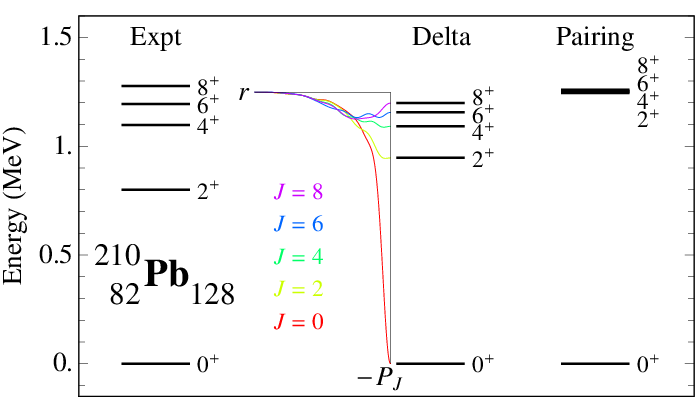
\includegraphics[width=0.6\textwidth]{figure/F_Pb210.png}
\caption{${}^{210}\textrm{Pb}$的低能实验能谱(左),对于一个zero-range delta的对应的能谱(中),以及对应于配对相互作用的能谱(右)。能级由它们的角动量和宇称$J^\pi$标记。插图显示了当两个中子在谐振子的$2g_{9/2}$轨道并且耦合的角动量为$J$时在距离$r$处发现这两个中子的几率密度$P_J$。\label{fig_Pb210}}
\end{figure}

配对相互作用由 Racah 为了原子中电子的分类而引入的。他能导出一个电子间的相互作用能的近似公式,并且可以证明配对相互作用的任意本征态都被一个'seniority 数'$v$表征,其对应于未配对耦合为轨道角动量$L=0$的电子数。Racah 最初对'seniority'的定义是利用分数的系数。后来,他指出可以利用群论来简化。Seniority 变成了在分类中与(酉)辛代数$Sp(2j+1)$相关的一个标记
\begin{equation}\label{eq_dif}
{\setlength\arraycolsep{3pt}\renewcommand{\arraystretch}{1}
\begin{array}{ccccc}
U(2j+1)&\supset&Sp(2j+1)&\supset&SU(2)\\
\downarrow& &\downarrow& &\downarrow\\
\textrm{[}1^{n}\textrm{]}& &[1^\upsilon]& &J
\end{array}}
\end{equation}
因为核子是全同的,$j^n$的配置所有态都属于完全反对称不可约表示$U(2j+1)$的$[1^n]$。因此,$Sp(2j+)$的不可约表示也一定是完全反对称的、属于$[1^\upsilon]$类型的,允许$senirority$的值为$\nu=n,n-2,\cdots,1$或0.

在定义\ref{eq_dif}中,seniority的出现作为与代数$Sp(2j+1)$相关的指标。这样的缺点是,依赖于$j$,代数可能是非常大的。问题可能变得更加复杂,当核子是非全同的,并且具有同位旋$t=\frac{1}{2}$。单粒子态的总数就变成了$\Omega\equiv(2j+1)(2t+1)$,很快就会遇到一个令人生畏的群理论的还原问题。幸运的是,一个更简单的可选择的seniority的定义可以通过代数学的语言给出,其不会随$j$改变。这个想法由Kerman(对于$t=0$的情况(即全同粒子))和Helmers(对于一般的$t$)同时且独立的提出来。其来源于产生和湮灭粒子的的$\widehat{S}_+^j$和$\widehat{S}_-^j$算符,以及具有第三类产生子$\widehat{S}^j_z$(有一个粒子产生同时有一个粒子湮灭的算符)的对易子。这一类算符的集合,即所谓的准自旋算符,在对易下封闭,并且形成(酉)辛代数(Sp(4t+2)),其可以被证明与$Sp(2j+1)$在分类\ref{eq_dif}中引入的的等同的性质。

配对问题的准自旋公式依赖于事实:配对相互作用是与$Sp(4t+2)$代数的二阶 Casimir 算符相关的。这允许对相同粒子$(t=0)$以及中子和质子$(t=\frac{1}{2})$的情况的本征值有个同时且简单的推导。这些年,许多结果都被推导出来了,并且考虑了许多在这两种情况下的扩展,其在下面进行单独的讨论。
\section{Identical nucleons}
对于$t=0$的情况,其包含了与$\textrm{SU}(2)$同构的代数Sp(2)。由于它与自旋代数有着形式上的相似性,“准自旋”这个名字是由Kerman创造的,而且这个术语适用于所有情况,即使$t\ne0$。准自旋代数Sp(2)\~SU(2)可以被得到,通过注意一点,在二次量子化中,在公式\ref{eq_eq8}中定义的配对相互作用被写为
\begin{equation}\label{eq_Vpair}
\widehat{V}_\textrm{pairing}=-g\widehat{S}^j_+\widehat{S}^j_-
\end{equation}
并且
\begin{equation}
\widehat{S}^j_+=\frac{1}{2}\sqrt{2j+1}(a_j^\dag\times a_j^\dag)^{(0)}_0,\quad\widehat{S}^j_-=\left(\widehat{S}^j_+\right)
\end{equation}
其中$a_{jm_j}^\dagger$在轨道$j$上产生一个投影为$m_j$的核子。不需要同位旋标记$t$和$m_t$来表征同类核子。符号$\times$表示角动量耦合,因此$\widehat{S}^j_+$创造了一对角动量耦合为$J=0$的核子。对易子$[\widehat{S}^j_+,\widehat{S}^j_-]\equiv2\widehat{S}^j_z$,和$[\widehat{S}^j_z,\widehat{S}^j_\pm]=\pm\widehat{S}^j_\pm$,表明$\widehat{S}^j_+$、$\widehat{S}^j_-$和$\widehat{S}^j_z$形成了一个封闭的代数SU(2).在SU(2)的基上可以导出几个标志性的结果。准自旋对称性允许配对相互作用的完整本征谱的确定,其由
\begin{equation}
\widehat{V}_\textrm{pairing}|j^nvJM_J\rangle=E(n,v)|j^nvJM_J\rangle
\end{equation}
和
\begin{equation}\label{eq_13}
E(n,v)=-\frac{g}{4}(n-v)(2j-n-v+3)
\end{equation}
给出。除了核子数$n$,总角动量$J$以及它的投影$M_J$以外,所有的本征态都通过一个seniority量子数$v$来表征,其表示没有在总角动量耦合为零的配对中的核子数。对于一个相互吸引的配对相互作用($g>0$),其具有最低能量的本征态,如果核子数为偶数时seniority$v=0$,,如果核子数为奇数时seniority$v=1$.这些最低能量的本征态,取决于归一化因子,对于偶数$n$可以被写成$(\widehat{S}^j_+)^{n/2}|0\rangle$,对于奇数$n$可以被写成$a_{jm_j}^\dag(\widehat{S}^j_+)^{n/2}|0\rangle$,其中$|0\rangle$是核子的真空态。

关于原子核配对关联的讨论,传统上是受到凝聚态超流性处理的启发,其是在1957年由Bardeen,Cooper和Schrieffer提出,并且后来被用来讨论原子核的配对(Bohr, Mttelson, \&Pines, 1958)。超流相的特征是在单个量子态中存在大量全同的玻色子。在超导体中的玻色子是在费米面处形成的具有相反动量的电子对,而在原子核中,根据前面的讨论,它们是具有相反角动量的价核子对。

这些概念的一般形式涉及到几个轨道。在简并轨道的情况下,这可以通过替换来实现$\widehat{S}_\mu^j\mapsto\widehat{S}_\mu\equiv\sum_j\widehat{S}^j_\mu$,这使得前面的所有结果对单$j$有效,保持不变。后面的公式可以应用于单幻核,但由于它需要配对相互作用与简并轨道的的假设,因此其适用性受到限制。

Richardson 在Bethe假设的基础上,提出了一种求解分布在非简并能级上的粒子间通过对力发生相互作用的问题的精确方法,并将其推广到其他可积配对模型中。Richardson 方法的证明可以通过用非简并单粒子能量补充配对相互作用\ref{eq_Vpair},以获得以下哈密顿量:
\begin{equation}\label{eq_hamilton4}
\widehat{H}_\textrm{pairing}=\sum_j\epsilon_j\widehat{n}_j-g\widehat{S}_+\widehat{S}_-
\end{equation}
其中$\widehat{n}_j$是轨道$j$的数量算符,$\epsilon_j$是轨道的单粒子能,并且$\widehat{S}_\pm=\sum_j\widehat{S}^j_\pm$。哈密顿量\ref{eq_hamilton4}的可解性来自于$\textrm{SU}(2)\bigotimes\textrm{SU}(2)\bigotimes\cdots$对称性,其中每一个$\textrm{SU}(2)$代数对应于一个特定的$j$。本征态的形式是
\begin{equation}\label{eq_prod}
\prod_{p=1}^{n/2}\left(\sum_j\frac{\widehat{S}_+^j}{2\epsilon_j-E_p}\right)|{\rm o}\rangle
\end{equation}
其中$E_p$是$n/2$耦合的解,非线性Richardson方程
\begin{equation}
\sum_j\frac{\Omega_j}{2\epsilon_j-E_p}-\sum_{p'(\ne p)}^{n/2}\frac{2}{E_{p'}-E_p}=\frac{1}{g},\quad p=1,\ldots,n/2
\end{equation}
其中$\Omega_j=j+1/2$。这个方程可以用图解的方式求解,图\ref{F_richardson}给出了一个简单的$n=2$的情况。在乘积\ref{eq_prod}中的每一对都通过依赖于能量$E_p$系数$\alpha_j=(2\epsilon_j-E_p)^{-1}$来定义,其中$p$标记$n/2$对。Bethe假设的一个特点是它不再由相同对的叠加组成,因为当$p$变换时,系数$(2\epsilon_j-E_p)^{-1}$从1变到$2/n$。因此,Richardson的模型提供了一个解,满足所有可能的从具有超流性质到具有很少或没有对关联性质的哈密顿量\ref{eq_hamilton4}。这个解能否被称为超流的取决于与强度$g$相关的差异$\epsilon_j-\epsilon_{j'}$。
\begin{figure}[H]
\centering
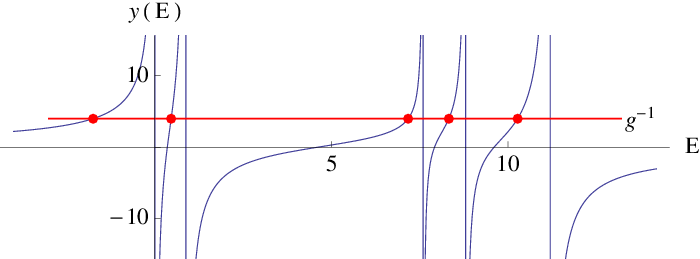
\includegraphics[width=0.6\textwidth]{figure/F_richardson.png}
\caption{两个核子在5个单粒子轨道上的分布的Richardson方程的图形解。求和$\Sigma_j\Omega_j/(2\epsilon_j-E)\equiv y(E)(\textrm{in MeV}^{-1})$作为$E$(in MeV)的函数被画出。该曲线(blue)与曲线${y=1/g}$(red)的交点(red dots)对应于Richardson方程的解。\label{F_richardson}}
\end{figure}


配对哈密顿量\ref{eq_hamilton4}允许非简并的单粒子轨道$\epsilon_j$,但是要求强度$g$是独于$j$的常数。或者,一个具有简并单粒子轨道的哈密顿量$\epsilon_j=\epsilon$,但是强度$g_j$是轨道依赖的
\begin{equation}
\widehat{H}'_\textrm{pairing}=\epsilon\sum_j\widehat{n}_j-\sum_jg_j\widehat{S}^j_+\sum_{j'}g_{j'}\widehat{S}^{j'}_-
\end{equation}
基于Bethe假设,其也能被精确求解。然而,对于具有任意非简并的单粒子轨道$\epsilon_j$和任意轨道相关强度$g_j$的配对哈密顿量,除了在两轨道的情况下,还没有确切的解。$\epsilon_j=g_j^2$的情况也是可解的,并且被应用在重核中。到目前为止,讨论都仅限于两个轨道$j$和$j'$之间的强度为$g_{jj'}$的可分离的相互作用,其中$g_{jj'}$的可被分解为$g_{jj'}=g_jg_{j'}$。不可分离的配对相互作用的精确解也可以通过结合运动的有理和双曲积分的得到,在综述(Dukelsky, Pittel, \& Sierra, 2004)有讨论这个问题。

尽管存在这些可能的推广,但应该记住,配对相互作用只是核子之间实际的残余相互作用的近似,如图\ref{fig_Pb210}所示。为了得到更加普适的方法,对壳模型的哈密顿量\ref{eq_hamilton3}考虑如下的条件:
\begin{equation}\label{eq_18}
[[\widehat{H}_{\rm GS},\widehat{S}_+^\alpha],\widehat{S}_+^\alpha]=\Delta\left(\widehat{S}^\alpha_+\right)^2
\end{equation}
其中$\Delta$是一个常数,$\widehat{S}_+^\alpha=\Sigma_j\alpha_j S_+^j$产生$\widehat{H}_{\rm GS}$的能量为$E_0$的最低的两粒子本征态,$\widehat{H}_{\rm GS}\widehat{S}_+^\alpha|{\rm}\rangle=E_0\widehat{S}_+^\alpha|{\rm}\rangle$。由Talmi提出的推广了的seniority的条件要比配对相互作用的假设要弱得多,并且它不需要对易子$[\widehat{S}_+^\alpha,\widehat{S}_-^\alpha]$产生(取决于一个常数)数量算符,这个算符是准自旋公式的核心。尽管没有一个封闭的代数结构,但是仍然有可能计算出满足条件\ref{eq_18}的哈密顿量的精确解。对于偶数个核子,它的基态具有与准自旋形式相同的简单结构
\begin{equation}
\widehat{H}_{\rm GS}\left(\widehat{S}_+^\alpha\right)^{n/2}|{\rm o}\rangle=E_{\rm GS}(n)\left(\widehat{S}_+^\alpha\right)^{n/2}|{\rm o}\rangle
\end{equation}
具有对应任意的核子数$n$都可以被计算得到的能量
\begin{equation}
E_{\rm GS}(n)=nE_0+\frac{1}{2}n(n-1)\Delta
\end{equation}
由于它是线性和二次依赖于核子数$n$的,所以这个结果可以被认为是一个Racah’s seniority公式\ref{eq_13}的推广,当$E_0=-g(j+1)/2$和$\Delta=g/2$时可以化简得到。

\subsection{Neutrons and protons}